\documentclass[a4paper,UTF8]{article}
\usepackage{ctex}
\usepackage[margin=1.25in]{geometry}
\usepackage{color}
\usepackage{graphicx}
\usepackage{amssymb}
\usepackage{amsmath}
\usepackage{amsthm}
\usepackage{enumerate}
\usepackage{bm}
\usepackage{hyperref}
\usepackage{pgfplots}
\usepackage{epsfig}
\usepackage{color}
\usepackage{tcolorbox}
\usepackage{mdframed}
\usepackage{lipsum}
\usepackage{natbib}
\newmdtheoremenv{thm-box}{myThm}
\newmdtheoremenv{prop-box}{Proposition}
\newmdtheoremenv{def-box}{定义}

\setlength{\evensidemargin}{.25in}
\setlength{\textwidth}{6in}
\setlength{\topmargin}{-0.5in}
\setlength{\topmargin}{-0.5in}
% \setlength{\textheight}{9.5in}
%%%%%%%%%%%%%%%%%%此处用于设置页眉页脚%%%%%%%%%%%%%%%%%%
\usepackage{fancyhdr}                                
\usepackage{lastpage}                                   
\usepackage{layout}                                     
\newtheorem*{solution}{Solution}

\footskip = 10pt 
\pagestyle{fancy}                    % 设置页眉                 
\lhead{2020年秋季}                    
\chead{高级机器学习}                                                
% \rhead{第\thepage/\pageref{LastPage}页} 
\rhead{作业二}                                                                                               
\cfoot{\thepage}                                                
\renewcommand{\headrulewidth}{1pt}  			%页眉线宽,设为0可以去页眉线
\setlength{\skip\footins}{0.5cm}    			%脚注与正文的距离           
\renewcommand{\footrulewidth}{0pt}  			%页脚线宽,设为0可以去页脚线

\makeatletter 									%设置双线页眉                                        
\def\headrule{{\if@fancyplain\let\headrulewidth\plainheadrulewidth\fi%
\hrule\@height 1.0pt \@width\headwidth\vskip1pt	%上面线为1pt粗  
\hrule\@height 0.5pt\@width\headwidth  			%下面0.5pt粗            
\vskip-2\headrulewidth\vskip-1pt}      			%两条线的距离1pt        
 \vspace{6mm}}     								%双线与下面正文之间的垂直间距              
\makeatother  

%%%%%%%%%%%%%%%%%%%%%%%%%%%%%%%%%%%%%%%%%%%%%%
\numberwithin{equation}{section}
%\usepackage[thmmarks, amsmath, thref]{ntheorem}
\newtheorem{myThm}{myThm}
\newtheorem*{myDef}{Definition}
\newtheorem*{mySol}{Solution}
\newtheorem*{myProof}{Proof}
\newtheorem*{myRemark}{备注}

\newcommand{\indep}{\rotatebox[origin=c]{90}{$\models$}}
\newcommand*\diff{\mathop{}\!\mathrm{d}}

\usepackage{multirow}

%--

%--
\begin{document}
\title{高级机器学习\\
作业二}
\author{丁豪\, 181220010} 
\maketitle
%%%%%%%% 注意: 使用XeLatex 编译可能会报错,请使用 pdfLaTex 编译 %%%%%%%

\section*{学术诚信}

本课程非常重视学术诚信规范,助教老师和助教同学将不遗余力地维护作业中的学术诚信规范的建立。希望所有选课学生能够对此予以重视。\footnote{参考尹一通老师\href{http://tcs.nju.edu.cn/wiki/}{高级算法课程}中对学术诚信的说明。}

\begin{tcolorbox}
	\begin{enumerate}
		\item[(1)] 允许同学之间的相互讨论,但是{\color{red}\textbf{署你名字的工作必须由你完成}},不允许直接照搬任何已有的材料,必须独立完成作业的书写过程;
		\item[(2)] 在完成作业过程中,对他人工作(出版物、互联网资料)中文本的直接照搬(包括原文的直接复制粘贴及语句的简单修改等)都将视为剽窃,剽窃者成绩将被取消。{\color{red}\textbf{对于完成作业中有关键作用的公开资料,应予以明显引用}};
		\item[(3)] 如果发现作业之间高度相似将被判定为互相抄袭行为,{\color{red}\textbf{抄袭和被抄袭双方的成绩都将被取消}}。因此请主动防止自己的作业被他人抄袭。
	\end{enumerate}
\end{tcolorbox}

\section*{作业提交注意事项}
\begin{tcolorbox}
	\begin{enumerate}
		\item[(1)] 请在LaTeX模板中{\color{red}\textbf{第一页填写个人的姓名、学号信息}};
		\item[(2)] 本次作业需提交该pdf文件、问题4可直接运行的源码,将以上几个文件压缩成zip文件后上传。zip文件格式为{\color{red}\textbf{学号.zip}},例如170000001.zip;pdf文件格式为{\color{red}\textbf{学号\_姓名.pdf}},例如170000001\_张三.pdf。
		\item[(3)] 未按照要求提交作业,或提交作业格式不正确,将会{\color{red}\textbf{被扣除部分作业分数}};
		\item[(4)] 本次作业提交截止时间为{\color{red}\textbf{12月25日23:59:59}}。除非有特殊情况(如因病缓交),否则截止时间后不接收作业,本次作业记零分。
	\end{enumerate}
\end{tcolorbox}

\newpage
\section{[20pts] PAC Learning for Finite Hypothesis Sets}
对于可分的有限假设空间,简单的~ERM~算法也可以导出~PAC~可学习性。请证明:

令~$\mathcal{H}$~为可分的有限假设空间, $D$~为包含~$m$~个从~$\mathcal{D}$~独立同分布采样所得的样本构成的训练集, 学习算法~$\mathfrak{L}$~基于训练集~$D$~返回与训练集一致的假设~$h_D$, 对于任意~$c\in \mathcal{H}$, $0<\epsilon, \delta < 1$, 如果有~$m \geq \frac{1}{\epsilon}(\ln|\mathcal{H}|+\ln\frac{1}{\delta})$, 则
\begin{equation}
    P\left(E(h_D)\leq\epsilon\right)\geq 1-\delta,
\end{equation}
即$E(h)\leq\epsilon$~以至少~$1-\delta$~的概率成立.

\noindent 提示:注意到~$h_D$~必然满足~$\widehat{E}_D(h_D) = 0$.

\begin{solution}
此处用于写解答(中英文均可)

由题目已知条件$$m\ge\frac 1 \epsilon(ln(|\mathcal H|)+\ln\frac 1 \delta)$$
可得$$|\mathcal H|e^{-m\epsilon} \le \delta$$
输出的假设$h_D$泛化误差大于$\epsilon$且在训练集上表现完美的概率,小于满足上述条件的所有假设出现概率之和(Union bound),同时又由于已知经验误差为0:
$$P(E(h_D)>\epsilon)=P(E(h_D)>\epsilon \land \widehat{E}_D(h_D)=0)$$
$$<P(h\in \mathcal H:E(h)>\epsilon\land \widehat{E}(h)=0)$$
$$<|\mathcal H|(1-\epsilon)^m<|\mathcal H|e^{-m\epsilon}\le\delta$$
所以
$$P(E(h_D)\le\epsilon)\ge1-P(E(h_D)>\epsilon)\ge 1-\delta$$
\end{solution}

\section{\textbf{[20pts]} semi-supervised learning}
	多标记图半监督学习算法~\citep{conf/nips/ZhouBLWS03}的正则化框架如下(另见西瓜书p303)。
\begin{equation}
\mathcal{Q}(F)=\frac{1}{2}\left(\sum_{i, j=1}^{n} W_{i j}\left\Vert\frac{1}{\sqrt{d_{i}}} F_{i}-\frac{1}{\sqrt{d_{j}}} F_{j}\right\Vert^{2}\right)+\mu \sum_{i=1}^{n}\left\|F_{i}-Y_{i}\right\|^{2}
\end{equation}
\begin{enumerate}
	\item  \textbf{[10pts]} 求正则化框架的最优解$F^*$。
	\item  \textbf{[10pts]}试说明该正则化框架与书中p303页多分类标记传播算法之间的关系。
\end{enumerate}

\begin{solution}
此处用于写解答(中英文均可)
\begin{enumerate}
\item 由于$Q(F)$为凸函数,因而求解$F^{*}$就是求解$\frac{\partial{Q(F)}}{\partial{F}} = 0$
\begin{equation*}
	\begin{split}
		\| \frac{1}{\sqrt{d_{i}}} F_{i} - \frac{1}{\sqrt{d_{j}}}F_{j} \|^{2} &= (\frac{1}{\sqrt{d_{i}}}F_{i} - \frac{1}{\sqrt{d_{j}}}F_{j})(\frac{1}{\sqrt{d_{i}}}F_{i} - \frac{1}{\sqrt{d_{j}}}F_{j})^{\top} \\
	&= \frac{1}{d_{i}}F_{i}F_{i}^{\top} - \frac{2}{\sqrt{d_{i}d_{j}}}F_{i}F_{j}^{\top} + \frac{1}{d_{j}}F_{j}F_{j}^{\top} \\
	\end{split}
\end{equation*}
​所以(2.1)式等号右边第一项可化为
\begin{equation*}
	\begin{split}
		&\quad \frac{1}{2}\left( \sum_{i,j}W_{ij} \| \frac{1}{\sqrt{d_{i}}}F_{i} - \frac{1}{\sqrt{d_{j}}}F_{j} \|^{2}  \right)\\
		&= \frac{1}{2}\left(\sum_{i=1}^{n}\sum_{j=1}^{n}W_{ij}(\frac{1}{d_{i}}F_{i}F_{i}^{\top} - \frac{2}{\sqrt{d_{i}d_{j}}}F_{i}F_{j}^{\top} + \frac{1}{d_{j}}F_{j}F_{j}^{\top}) \right)\\
		&= \frac{1}{2}\left( \sum_{i=1}^{n}\sum_{j=1}^{n}\frac{W_{ij}}{d_i}F_{i}F_{i}^{\top} - 2\sum_{i=1}^{n}\sum_{j=1}^{n}W_{ij}F_{i}F_{j}^{\top}\frac{1}{\sqrt{d_{i}d_{j}}} + \sum_{i=1}\sum_{j=1}\frac{W_{ij}}{d_j}F_{j}F_{j}^{\top} \right) \\
		&=  \frac{1}{2}\left( \sum_{i=1}^{n}F_{i}F_{i}^{T} - 2\sum_{i=1}^{n}\sum_{j=1}^{n}W_{ij}F_{i}F_{j}^{\top}\frac{1}{\sqrt{d_{i}d_{j}}} + \sum_{j=1}^{n}F_{j}F_{j}^{\top}
		\right) \\
		&= 	\frac{1}{2}\left( 2\sum_{i=1}^{n}\|F_{i}^{2}\| - 2\sum_{i=1}^{n}\sum_{j=1}^{n}W_{ij}F_{i}F_{j}^{\top}\frac{1}{\sqrt{d_{i}d_{j}}}  \right) \\
		&= tr(F^{T}F) - \sum_{i=1}^{n}\sum_{j=1}^{n}W_{ij}F_{i}F_{j}^{\top}\frac{1}{\sqrt{d_{i}d_{j}}}
	\end{split}
\end{equation*}
由于标记传播矩阵有$$S = D^{-\frac{1}{2}}WD^{-\frac{1}{2}}$$
​故$$(S_{ij}) = \frac{1}{\sqrt{d_{i}d_{j}}}W_{ij}$$
所以有$$\sum_{i=1}^{n}\sum_{j=1}^{n}\frac{W_{ij}}{\sqrt{d_{i}d_{j}}}F_{i}F_{j}^{\top} = \sum_{i=1}^{n}\sum_{j=1}^{n}S_{ij}F_{i}F_{j}^{\top}=tr(SFF^{\top})$$

​而(2.1)式等号右边第二项为
$$\sum_{i=1}^{n}\|F_{i} - Y_{i} \|^{2} = \sum_{i=1}^{n} \| (F-Y)_{i}\|^{2} = \| F - Y\|^{2}_{\mathcal{F}}$$
​综上,有
$$Q(F) = tr(F^{\top}F) - tr(SFF^{\top}) + \mu \| F - Y\|^{2}_{\mathcal{F}}$$
令
\begin{equation*}
	\begin{split}
		\frac{\partial{Q(F)}}{\partial{F}} &= 2F - (SF + S^{\top}F) + 2\mu(F-Y) \\
		&= 2(I - S + \mu I)F - 2\mu Y\\
		&=0
	\end{split}
\end{equation*}
解得
\begin{equation*}
	\begin{split}
		F^{*} &= (I - S + \mu I)^{-1}Y \\
		&= \left[(1+\mu)I - S\right]\mu Y \\
		&= \mu\left[(1+\mu)I -S \right]^{-1}Y
	\end{split}
\end{equation*}
\item 考虑西瓜书p303页中多分类表及传播算法的收敛解
$$F^{*} = (1-\alpha)(I - \alpha S)^{-1}Y$$
而我们在第一问中求得的最优解为
\begin{equation*}
	\begin{split}
		F^{*} &= \mu\left[(1+\mu)I -S \right]^{-1}Y\\
		&=\frac{\mu}{1+\mu} \left[I - \frac{1}{1+\mu}S\right]^{-1} Y\\
		&=(1-\frac{1}{1+\mu})\left[I - \frac{1}{1+\mu}S\right]^{-1} Y
	\end{split}
\end{equation*}
不难发现,当$\alpha=\frac{1}{1+\mu}$时,二者收敛解一致。
\end{enumerate}
\end{solution}



\section{\textbf{[30pts]} Mixture Models}
一个由K个组分(component)构成的多维高斯混合模型的概率密度函数如下:
\begin{equation}
    p\left(\boldsymbol{x}\right) = \sum_{k=1}^{K} P\left(z=k\right) p\left(\boldsymbol{x}|\boldsymbol{\mu}_k,\boldsymbol{\Sigma}_k\right)
\end{equation}
其中$z$是隐变量,$P(z)$表示K维离散分布,其参数为$\boldsymbol{\pi}$,即$p\left(z=k\right) = \pi_k$。$p\left(\boldsymbol{x}|\boldsymbol{\mu}_k,\boldsymbol{\Sigma}_k\right)$表示参数为$\boldsymbol{\mu}_k,\boldsymbol{\Sigma}_k$的多维高斯分布。
\begin{enumerate}
    \item  \textbf{[10pts]} 请使用盘式记法表示高斯混合模型。
    \item \textbf{[10pts]} 考虑高斯混合模型的一个具体的情形,其中各个分量的协方差矩阵$\boldsymbol{\Sigma}_k$全部被
限制为一个共同的值$\boldsymbol{\Sigma}$。求EM算法下参数$\pi_k,\boldsymbol{\mu}_k,\boldsymbol{\Sigma}$的更新公式。
\item \textbf{[10pts]} 考虑一个由下面的混合概率分布给出的概率密度模型:
\begin{equation}
    p\left(\boldsymbol{x}\right) = \sum_{k=1}^{K} \pi_k p\left(\boldsymbol{x}| k\right)
\end{equation}
并且假设我们将$\boldsymbol{x}$划分为两部分,即$\boldsymbol{x} = \left(\boldsymbol{x}_a,\boldsymbol{x}_b\right)$。证明条件概率分布$p\left(\boldsymbol{x}_a|\boldsymbol{x}_b\right)$本身是一个混合概率分布。求混合系数以及分量概率密度的表达式。(注意此题没有规定$p\left(\boldsymbol{x}|k\right)$的具体形式)
\end{enumerate}
\begin{solution}
此处用于写解答(中英文均可)
\begin{enumerate}

\item 设可观测变量集为$X=\{x_1,x_2,\dots,x_N\}$,则高斯混合模型的盘式记法

\centerline{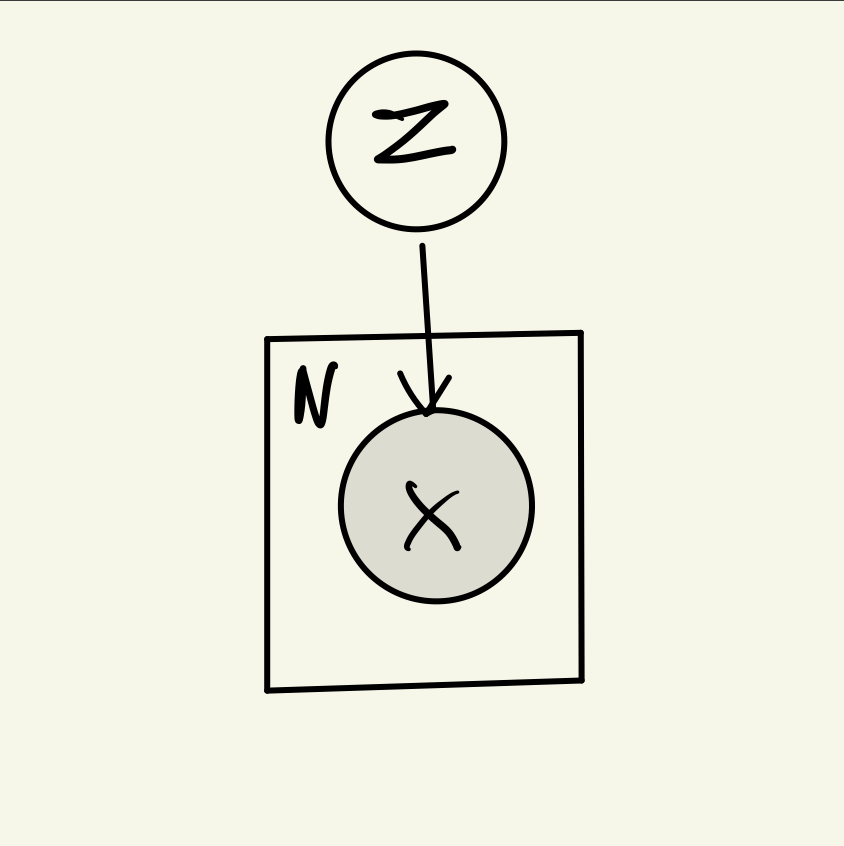
\includegraphics[scale = 0.3]{4.1.png}}

\item 在E步,根据已知参数推断隐变量$z$的分布
$$p(x)=\prod_{n=1}^N p(x_n)=\prod_{n=1}^N\sum_{k=1}^K\pi_k p(x_n|\mu_k,\Sigma)$$
对数似然函数:
$$L(x)=\ln p(x|\pi,\mu,\Sigma)=\sum_{n=1}^N\ln\left(\sum_{k=1}^K\pi_k p(x_n|\mu_k,\Sigma)\right)$$
在M步最大化对数似然函数,有:\\
a)对$\mu_k$求极大:
$$\frac{\partial L(x)}{\partial \mu_k}=\sum_{n=1}^N\ln\left(\frac{\pi_k p(x_n|\mu_k,\Sigma)}{\sum_{j=1}^K\pi_j p(x_n|\mu_j,\Sigma)}\right)\Sigma^{-1}(x_n-\mu_k)=0$$
令:
$$\gamma(z_{nk})=\frac{\pi_k p(x_n|\mu_k,\Sigma)}{\sum_{j=1}^K\pi_j p(x_n|\mu_j,\Sigma)}$$
$$N_k=\sum_{n=1}^N\gamma(z_{nk})$$
则上式解得:
$$\mu_k=\frac 1 {N_k}\sum_{n=1}^N\gamma(z_{nk})x_n$$
b)对$\Sigma$求极大:
$$\frac{\partial L(x)}{\partial \Sigma}=\frac 1 2 \sum_{n=1}^N\sum_{k=1}^K\gamma(z_{nk})\left(\Sigma^{-1}(x_n-\mu_k)(x_n-\mu_k)^\top\Sigma^{-1}-\Sigma^{-1}\right)=0$$
等式两边同时乘两次$\Sigma$
$$\sum_{n=1}^N\sum_{k=1}^K\gamma(z_{nk})\left((x_n-\mu_k)(x_n-\mu_k)^\top-\Sigma\right)=0$$
得
$$\Sigma=\frac 1 N\sum_{n=1}^N\sum_{k=1}^K\gamma(z_{nk})(x_n-\mu_k)(x_n-\mu_k)^\top$$
c)对$\pi_k$求极大。由于$\pi$为概率分布,需要满足$\sum_k \pi_k=1$条件,因此引入拉格朗日项以及系数$\lambda$:
$$L'(x)=L(x)+\lambda(\sum_{k=1}^K-1)$$
$$\frac{\partial L'(x)}{\partial \pi_k}=\sum_{n=1}^N\frac{p(x_n|\mu_k,\Sigma)}{\sum_{j=1}^K\pi_jp(x_n|\mu_j,\Sigma)}=0$$
等式两侧同时乘$\pi_k$得
$$N_k+\lambda\pi_k=0$$
又由于$\sum_k \pi_k=1$所以有$\sum_k \frac {-N_k}{\lambda}=1 \implies \lambda = -\sum_{n=1}^N\left(  \frac{\sum_{k=1}^K\pi_k p(x_n|\mu_k,\Sigma)}{\sum_{j=1}^K\pi_j p(x_n|\mu_j,\Sigma)}\right)=-N$

所以$$\pi_k=\frac{N_k}{N}$$

\item 
\begin{equation*}
\begin{split}
	p(x_a|x_b) &= \frac{p(x_a,x_b)}{p(x_b)}\\
	&=\frac{p(x)}{p(x_b)}\\
	&=\frac{\sum_{k=1}^K\pi_kp(x|k)}{x_b}\\
	&=\frac{\sum_{k=1}^K\pi_kp(x_a,x_b|k)}{x_b}\\
	&=\sum_{k=1}^K\pi_k \frac{p(x_b|k)}{p(x_b)}\frac{p(x_a,x_b|k)}{p(x_b|k)}\\
	&=\sum_{k=1}^K\pi_k \frac{p(x_b|k)}{p(x_b)}p(x_a|x_b,k)
\end{split}	
\end{equation*}
故可以将其表示为混合概率分布,其中混合系数为:
$$\frac{\pi_kp(x_b|k)}{p(x_b)}=\frac{\pi_k\sum_{x_a'}p(x_a',x_b|k)}{\sum_{k'=1}^K\pi_{k'}\sum_{x_a'}p(x_a',x_b|k')}$$
分量概率密度为:
$$p(x_a|x_b,k)$$
\end{enumerate}
\end{solution}

\section{\textbf{[30pts]}Latent Dirichlet Allocation}
我们提供了一个包含$8888$条新闻的数据集\texttt{news.txt.zip},该数据集中每一行是一条新闻。在该数据集上完成LDA模型的使用及实现。

数据预处理提示:你可能需要完成分词及去掉一些停用词等预处理工作。

在本题中需要完成:
\begin{enumerate}
    \item \textbf{[10pts]}使用开源的LDA库(如scikit-learn),计算给出$K=\{5, 10, 20\}$个话题时,每个话题下概率最大的10个词及其概率。
    \item \textbf{[20pts]}不借助开源库,手动实现LDA模型,计算给出$K=\{5, 10, 20\}$个话题时,每个话题下概率最大的10个词及其概率。
\end{enumerate}
注:需要在报告中描述模型计算的结果,以及如何复现自己的结果,提交的作业中至少应该包含\texttt{lda\_use.py}和\texttt{lda.py}两个文件,分别为使用和不使用第三方库的源码。
\begin{solution}
	数据加载段两者相同。

	首先将news.txt中每一行的英文文本数据进行“小写化”,“去标点”,“去停用词”三步数据预处理。然后将预处理完毕的8888条文本进行进一步操作:
\begin{enumerate}
	\item 使用sklearn.feature\_extraction.text.CountVectorizer基于上一步产生的标准文本统计词频,生成“词袋模型”。然后使用sklearn.decomposition.LatentDirichletAllocation构造LDA模型,并使用其fit\_transform方法直接针对上一步产生的“词袋模型”进行拟合。最终,输出其参数components\_中我们所需要的每一类的前10个高频词以及其概率(某类中某词的频率除以此类中总词频率得到)。最终在进行10轮全文Gibss迭代之后的结果见文件“实验记录.md”
	\item 首先手动实现了“词袋模型”的统计生成。然后,实现了基于Gibbs采样的LDA模型,模型具有超参数$\alpha,\beta$分别用于控制文章中的主题密度、主题中的单词密度,由于实验条件限制(运行、对比代价太大),因而直接指定为常数5和0.1且不再调参。\\
		  每次Gibss采样的具体过程为:
		  \begin{enumerate}
			  \item 首先按照初始分布给每篇文档的每一个词,分配主题
			  \item 每次迭代排除当前词的旧主题,然后根据其他词的出现频率来估计当前词属于不同主题的概率,按照此概率重新为这个词采样得到新主题。用同样的方法不断更新下一个词的主题,直到收敛条件(这里是指定的迭代轮数)。在迭代的过程中,我们维护三个量:1)每篇文章
			  \item 最终,我们可以根据维护的“每个主题每个词的出现次数”来计算得到每个主题下词频最高的10个词以及其出现频率。
		\end{enumerate}
		最终在进行10轮全文Gibss迭代之后的结果见文件“实验记录.md”\\
		第1题与第2题在实验阶段使用谷歌提供的co-lab平台进行开发,最终将笔记本转化为.py文件,分别位于"lda\_use.py"以及"lda.py",计算结果已经使用随机种子"2020"进行固定,直接
		运行即可复现结果。
\end{enumerate}
\end{solution}
\newpage
\bibliography{ref}
参考资料
\begin{enumerate}
	\item 掉包使用LDA模型参考了:https://www.cnblogs.com/pinard/p/6908150.html。主要是学习了包的基础用法以及可调参数。
	\item 手动实现LDA模型参考了:https://github.com/nkoilada/lda。其“吉布斯采样”部分的实现非常具有启发性。
\end{enumerate}
\bibliographystyle{abbrvnat}
\end{document}